
\section{Motivation}

The rapid growth of data generated by large-scale information systems leads to new opportunities for  society and businesses.
In order to turn the massive amount of data into value, efficient techniques are needed, that are able to extract useful information.
The generated value comes in different forms, for example visualizations, models, aggregated data or predictions can be of interest. 

A remarkable subset of this data is described as \textit{event data}, which is generated by \textit{process-aware information systems} in order to manage, execute and monitor business processes \cite{DBLP:journals/topnoc/Aalst09}.
With the non stopping rise of digitization of business processes more and more event data becomes utilizable, thus the potential value of this data is exploding.

The scientific engagement aiming to discover, analyze and improve real processes using event data led to \textit{process mining}. Process mining bridges the gab between the data-driven characteristic of data science and the process-centric view of process science \cite{DBLP:books/sp/Aalst16}.
The ongoing success of progress mining in research has been transferred to businesses, that successfully offer or utilize this technology.
Celonis, which is often considered as one of the biggest commercial providers of process mining, has been valued 2.5 billion dollar only 9 years after the company was founded \cite{celonis}.

Modern process mining software tends to focus on continuous analysis rather than the traditional offline and project-based approaches.
These business process monitoring systems are a key success factor for many organizations, since they allow to understand and supervise all connected processes of a company in real-time as the data is flowing.
The core idea of this approach is to automate process mining and keep a persistent connecting between the business process data and the analytical capabilities.

\begin{figure}[htbp!]
	\centering
	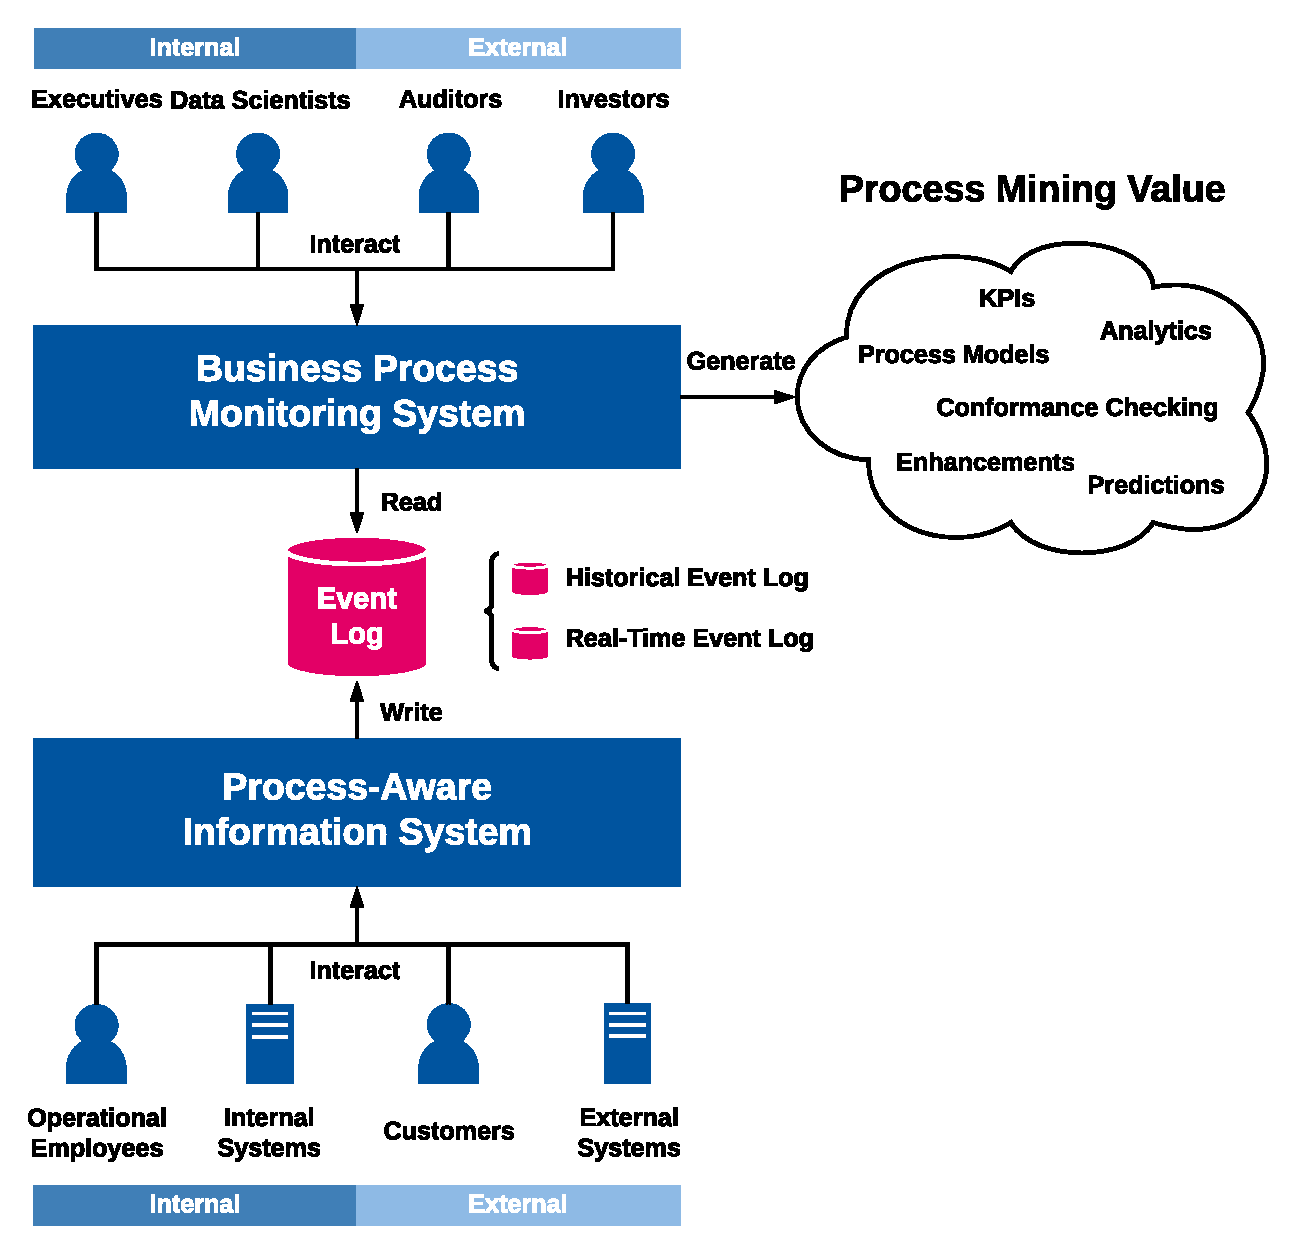
\includegraphics[width=\textwidth]{figures/process-monitoring}
	\caption{Business process monitoring allows to continuously apply process mining techniques in an automated fashion in order to generate value for internal and external process stakeholders.}
	\label{fig:process-monitoring}
\end{figure}

However, traditional process mining tends to be backward-looking  \cite{DBLP:conf/scsc/Aalst18}, i.e. it rather focuses on answering the question "What did happen?", rather than "What will happen?" or even "What should be done?".
Therefore, new techniques are required to add the forward-perspective to process mining software.

\section{Problem Statement}

Businesses can develop a competitive advantage, if their process mining software has predictive capabilities, that allow to predict the future of a running process instance.
For example, if it is known beforehand that a running process instance will probably exceed its deadline, measures can be initiated before damage occurs.
Furthermore, information about the next event or the future path of process instance can be of interest.
In some scenarios, processes instances have an outcome like success/failure or accepted/declined that can be predicted.

Precisely, given an event log with past executions of a process and a running (i.e. not completed) process instance, we would like to answer the following questions:

\begin{itemize}
	\item What will happen next?
	\item When will it happen?
	\item What is the most likely future path of the instance?
	\item When will the instance finish?
	\item What is the outcome of the instance?
\end{itemize}



\section{Research Goals}

This thesis aims to improve current state-of-art approaches for process prediction to improve the capabilities of process monitoring software.
The main research goal is to design, implement and evaluate a predictive model for event data that is able to take advantage of additional attribute and textual data associated with each event.
Since most current approach are not able to handle textual data, we would like to know to which extend textual data can improve the quality of process prediction.
Furthermore, we want to evaluate different design choices for a text-aware process prediction model and point out potential trade-offs.

\section{Contribution}



\section{Thesis Structure}

This thesis is structured in seven chapters.
In Chapter \ref{chap:prelim} the notations, definitions and concepts used in this contribution are introduced.
Chapter \ref{chap:related_work} summarizes relevant scientific contributions which focus on the problem of prediction in process mining to give an overview of already available methods and their capabilities.
A novel text-aware process prediction model is presented in Chapter \ref{chap:concept}.
Moreover, the details regarding the implementation of the model are given in Chapter \ref{chap:impl}.
In Chapter \ref{chap:eval} the performance of the model is evaluated and compared to current state-of-the-art prediction methods.
Finally, in Chapter \ref{chap:conclusion} a conclusion about all findings and an outlook towards future potential research on process prediction is given.